\documentclass[12pt,a4]{article}\usepackage[]{graphicx}\usepackage[]{xcolor}
% maxwidth is the original width if it is less than linewidth
% otherwise use linewidth (to make sure the graphics do not exceed the margin)
\makeatletter
\def\maxwidth{ %
  \ifdim\Gin@nat@width>\linewidth
    \linewidth
  \else
    \Gin@nat@width
  \fi
}
\makeatother

\definecolor{fgcolor}{rgb}{0.345, 0.345, 0.345}
\newcommand{\hlnum}[1]{\textcolor[rgb]{0.686,0.059,0.569}{#1}}%
\newcommand{\hlstr}[1]{\textcolor[rgb]{0.192,0.494,0.8}{#1}}%
\newcommand{\hlcom}[1]{\textcolor[rgb]{0.678,0.584,0.686}{\textit{#1}}}%
\newcommand{\hlopt}[1]{\textcolor[rgb]{0,0,0}{#1}}%
\newcommand{\hlstd}[1]{\textcolor[rgb]{0.345,0.345,0.345}{#1}}%
\newcommand{\hlkwa}[1]{\textcolor[rgb]{0.161,0.373,0.58}{\textbf{#1}}}%
\newcommand{\hlkwb}[1]{\textcolor[rgb]{0.69,0.353,0.396}{#1}}%
\newcommand{\hlkwc}[1]{\textcolor[rgb]{0.333,0.667,0.333}{#1}}%
\newcommand{\hlkwd}[1]{\textcolor[rgb]{0.737,0.353,0.396}{\textbf{#1}}}%
\let\hlipl\hlkwb

\usepackage{framed}
\makeatletter
\newenvironment{kframe}{%
 \def\at@end@of@kframe{}%
 \ifinner\ifhmode%
  \def\at@end@of@kframe{\end{minipage}}%
  \begin{minipage}{\columnwidth}%
 \fi\fi%
 \def\FrameCommand##1{\hskip\@totalleftmargin \hskip-\fboxsep
 \colorbox{shadecolor}{##1}\hskip-\fboxsep
     % There is no \\@totalrightmargin, so:
     \hskip-\linewidth \hskip-\@totalleftmargin \hskip\columnwidth}%
 \MakeFramed {\advance\hsize-\width
   \@totalleftmargin\z@ \linewidth\hsize
   \@setminipage}}%
 {\par\unskip\endMakeFramed%
 \at@end@of@kframe}
\makeatother

\definecolor{shadecolor}{rgb}{.97, .97, .97}
\definecolor{messagecolor}{rgb}{0, 0, 0}
\definecolor{warningcolor}{rgb}{1, 0, 1}
\definecolor{errorcolor}{rgb}{1, 0, 0}
\newenvironment{knitrout}{}{} % an empty environment to be redefined in TeX

\usepackage{alltt}

% ---- Metadata ---- %

\title{Honesty by Convenience: Corruption Tolerance in Ecuador}
\author{Daniel Sánchez}
\date{June 2022}

% ---- Load Packages ---- %

% Math

\usepackage{savesym} % Need to "save" the command that is already defined \varTheta

\usepackage{amsmath}
  \savesymbol{varTheta} 

% Fonts

% To set the TNR font for both text and equations:

\usepackage{mathspec}
  \setallmainfonts(Digits,Greek,Latin){Times New Roman}
\restoresymbol{MTP}{varTheta}

% Formatting

\usepackage{setspace}
  \doublespacing

\usepackage[margin = 1in]{geometry}

\usepackage{lscape}

% Setting the size of the section titles

\usepackage{titlesec}

\titleformat*{\section}{\normalsize\bfseries}

% Citation & Bibliographies

\usepackage[backend = biber, style = apa, citestyle = apa]{biblatex}
  \addbibresource{refs.bib}
  
% For tables:

 % For the modelsummary tables:
\usepackage{siunitx}
\usepackage{booktabs} 
  \newcolumntype{d}{S[input-symbols = ()]}
\usepackage{multirow}
\usepackage[flushleft]{threeparttable}

% For figure and table captions

\usepackage{caption}
  \captionsetup{labelfont = bf} % All in bold  
  
% Other packages

\usepackage{csquotes} % For quotation marks

\usepackage{epigraph} % For epigraph
  \setlength\epigraphwidth{9cm}
  \setlength\epigraphrule{1pt}

\usepackage{float} % For the H float option- only used in emergencies (lol)

\usepackage{textcomp} % For the registered trademark symbol.

% Always load these packages at the end of the preamble:

\usepackage{hyperref}

% ---- R Stuff to be used in the whole document ----

% Here I will execute or source R code through chunks that I need to use throughout the whole document.

% General settings



% Load the data by sourcing the data manipulation script. Note that survey design objects are indeed created in this script.
% We use the time argument in the chunks to reread or rerun the chunk in case external files are updated and chunks need to be rerun and re-cached.


% Perform all survey-robust tabulations by sourcing the R Script. 
% These are used on the text later.


% Run the first models


\IfFileExists{upquote.sty}{\usepackage{upquote}}{}
\begin{document}

% ---- Sections ---- %

% Abstract Child Document


% Abstract .Rnw File


\begin{center}
\textbf{
Honesty by Convenience: Corruption Tolerance in Ecuador\\
Daniel Sánchez}
\end{center}

\textit{
Attitudes towards corruption may be a strong determinant of its incidence. Using survey
data from the AmericasBarometer (AB), binary-outcome empirical models are estimated to discover
the key determinants of an increase in corruption tolerance in Ecuador between 2014 and
2016. It is found that two key variables may have influenced this increase. People who approved
of the President’s job performance initially justified bribes less, but by 2016 supporters justified corruption more. Also, those who identified closer to the political right justified corruption more in 2016. The jump is explained through these variables as the percentage of people who approved of the President decreased and the percentage of people identifying with the right increased. It is also found that the people who were either employed or outside the labor force justified bribes more in 2016 when compared to those who were unemployed.}

% Introduction Child Document


% Introduction .Rnw File


\section{Introduction}
\enquote{Even if you are from [my political party], I will fulfill my duties. If you steal, steal well!  Justify well! But do not let your affairs be seen, comrades\footnote{Translated from Cerda, 2021 in \cite[para. 2]{PlanV.2021}}}. Uttered publicly by Rosa Cerda, Ecuadorian congresswoman for the Napo province \parencite{Castro.2021}, these comments met widespread criticism around the country, although the remarks were initially met by cheers from the audience she addressed. However, Cerda's declarations did not transcend an eight day suspension \parencite{Ordonez.2021} and the whole event was soon forgotten by most citizens. 

This episode is only one of many corruption-related scandals that have happened in Ecuador, a middle-income country in South America. The country has seen increased COVID-19 vaccine inequality \parencite{Taj.2021}, weakened public health services \parencite{Celi.2020}, policymakers charging fees for political positions \parencite{Espinosa.2021}, lost Social Security funds \parencite{Pesantes.9152020}, a convicted former president as well as two vice-presidents impeached and removed on charges of corruption \parencite{Cabrera.2020}, among others. However, it is almost as if these no longer cause outrage: at most, they cause a sigh of disappointment or social media outrage which dwindles shortly after.

This apparent ambivalence has seen Ecuador place well above the corruption median in the world according to both Transparency International's and the World Bank's corruption indexes. About 90\% of voting-age Ecuadorians believe that at least half of politicians are corrupt and more than a quarter of them admit having been involved with bribes in 2019, according to the AmericasBarometer (AB) survey, by the Latin American Public Opinion Project (LAPOP). However, a mere 8.08\% consider that corruption is the most serious problem faced by the country and in fact 25.38\% of Ecuadorians believe that paying a bribe is justified. Further, tolerance to corruption has risen 11.79 percentage points from 2014 to 2019. Furthermore, Figure \ref{fig:ctolmap} shows that Ecuador is also one of the countries with the highest corruption tolerance in the region.

% Corruption Tolerance Choropleth Map based on 2019 values

% Sorry, this map was done with the paid AmericasBarometer databases, so I cannot actually put my source code and have it executed by KNITR. USFQ students are free to access another version of the document, they must only email me. Third parties must wait until I do it with the free databases. Check out hbc-v2 for some more info.

\begin{figure}[htbp]
  \label{fig:ctolmap}
      \caption{Corruption Tolerance (\%) Choropleth Map in 2019}
    \begin{center}
    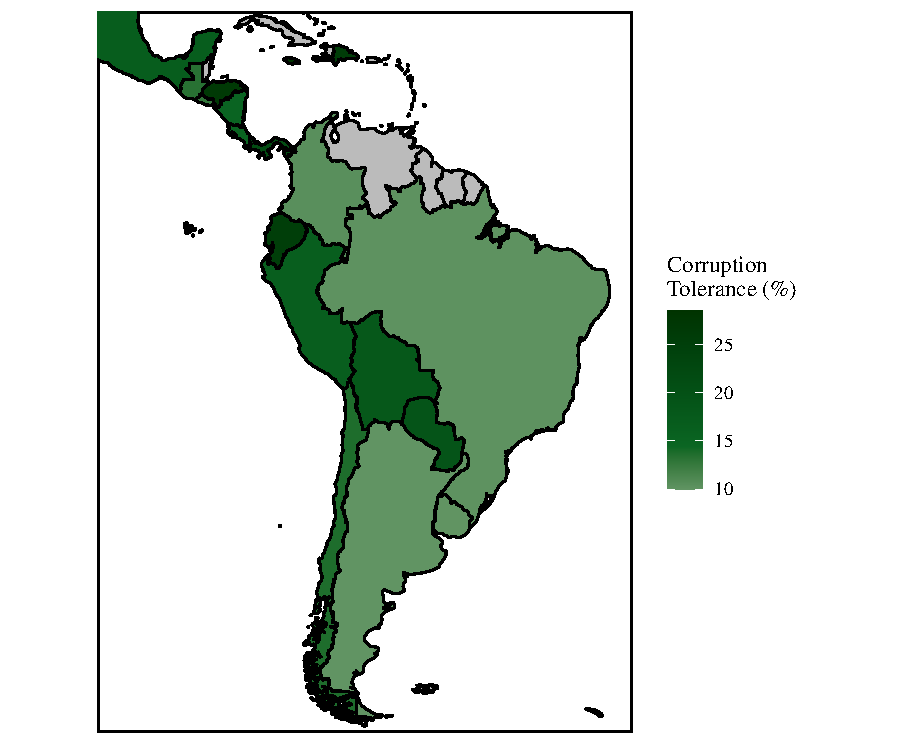
\includegraphics{images/ctol_map.pdf}
    \end{center}

A choropleth map showing corruption tolerance percentages across Latin America in 2019, where Ecuador places third in the most corruption tolerant countries. Darker areas imply higher percentages of corruption tolerance. Figure prepared by the author with data from the \textregistered AmericasBarometer 2018/19. 
\end{figure}

This paper aims to investigate the determinants of the largest corruption tolerance increase in Ecuador, seen from 2014 to 2016, as it can be seen in Figure \ref{fig:ctoly}. This period coincided with two key events in the country. First, the popularity of the governing regime sharply dropped for the first time in a decade \parencite{Quillupangui.2016}. Second, the country faced an economic recession \parencite{Weisbrot.2017}. The present paper will seek to relate  This is done by estimating a binary-outcome model through logistic regression, which relates the probability of tolerating corruption to several individual-level public opinion and economic indicators using the data from the AB. It is determined that changes in presidential job approval as well as in political wing preferences during the 2014 and 2016 period could have influenced the corruption tolerance increase. It is also found that those not unemployed justified corruption more in 2016 relative to those who were unemployed.

% Corruption Tolerance Time Series Graph

\begin{figure}[htbp]
\label{fig:ctoly}
\caption{Percent of Ecuadorians who justify corruption, by year}
\begin{knitrout}
\definecolor{shadecolor}{rgb}{0.969, 0.969, 0.969}\color{fgcolor}

{\centering 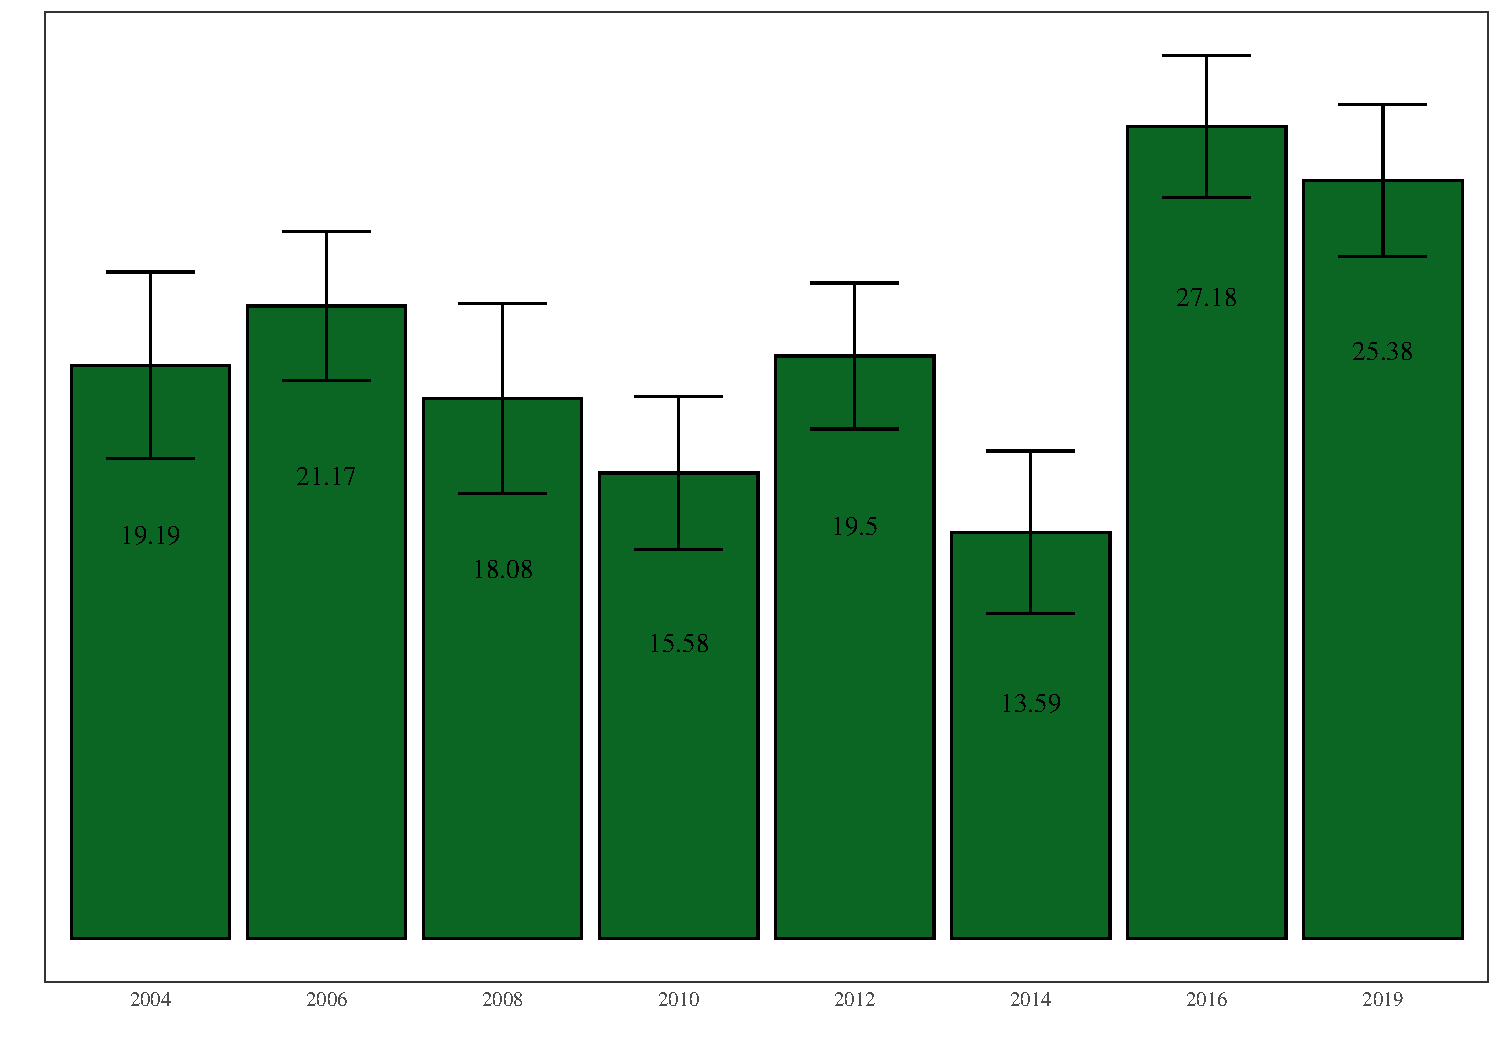
\includegraphics[width=\maxwidth]{figure/ctol_graph-1} 

}


\end{knitrout}


The evolution of corruption tolerance for Ecuador. The largest increase is seen from 2014 to 2016. Error bars show 95\% confidence intervals, considering survey design effects. Figure prepared by the author, with the open-access AB data.
\end{figure}

Changes to the attitudes toward corruption can be important for studying corruption incidence. A higher degree of corruption tolerance will eventually lead to larger corruption environments \parencite{Campbell.2014}. Learning what drives corruption tolerance can then foster better policymaking and citizen attitudes which steers individuals away from becoming involved in corruption.

The rest of the paper proceeds as follows. The following section gives an institutional and historical background of the paper's setting, Ecuador. Section 3 reviews the relevant literature. Section 4 develops the empirical methodology. Section 5 reviews the results from the empirical estimation. Section 6 discusses these results, and Section 7 concludes. 

% Institutional Background Child Document


% Context .Rnw File

\section{Institutional and Historical Background}
\label{sec:background}

As pointed out previously, the corruption tolerance increase happened at the same time as other key events. First, AB indicators denote a political crisis, as support for President Rafael Correa's regime took a sharp hit. Second, a recession hit Ecuador due to a commodity price collapse, an earthquake and other circumstances. Below, Figure \ref{fig:ecua_pol} shows several public opinion indicators and Figure \ref{fig:ecua_ec} displays economic conditions, both observed and perceived from 2014 to 2019. 
% Create the data to be used for the political opinion variables:

% Now do the graph
\begin{figure}[htbp]
\centering
\fbox{
\begin{minipage}{\textwidth}
\caption{Ecuadorian public opinion indicators, 2004-2019}
\label{fig:ecua_pol}
\begin{knitrout}
\definecolor{shadecolor}{rgb}{0.969, 0.969, 0.969}\color{fgcolor}

{\centering 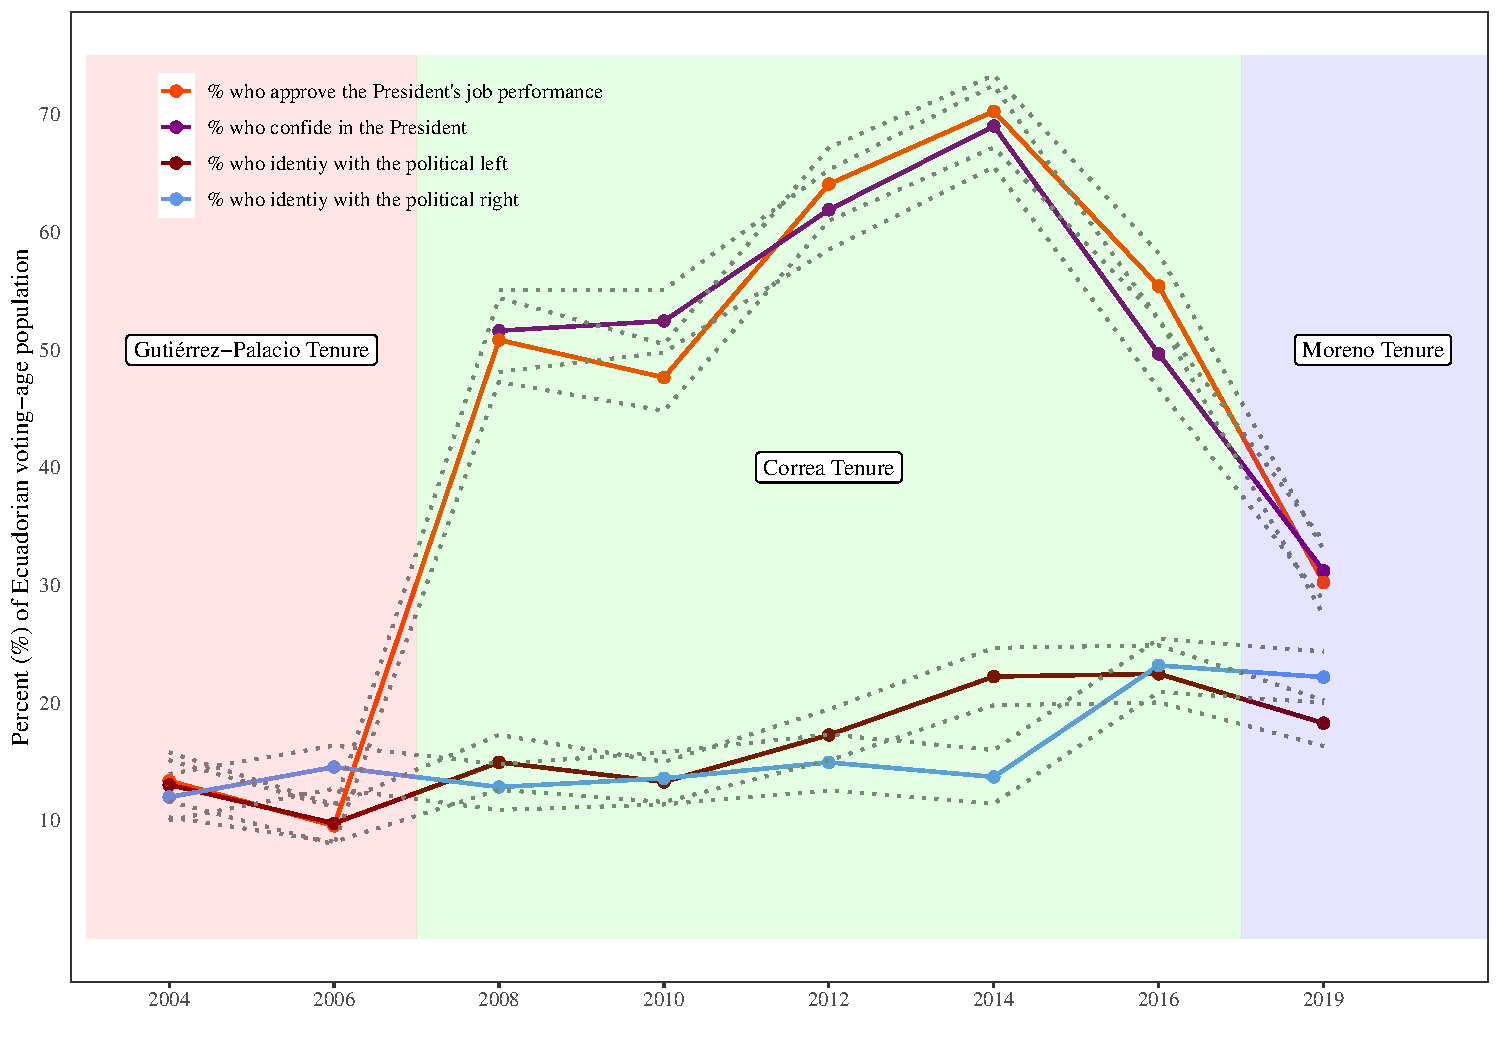
\includegraphics[width=\maxwidth]{figure/political_graph-1} 

}


\end{knitrout}
\textbf{Note:} The graph shows time series for political public opinion questions asked in the AB. Percentages are estimated as explained in \hyperref[app:first]{Appendix A} and error bars show 95\% confidence intervals considering design effects. Figure prepared by the author. \end{minipage}
}
\end{figure}

The AB data shows that indeed the President reached an all-time high popularity in 2014 and then a severe drop in 2016. This is seen through the percent of people who approve the President's job performance and the percent who report confidence in him. Another notable change in the political landscape is the way that voting-age population politically identified. There was a strong increase of the people who identified as the \enquote{right}, while those who identified with the \enquote{left} did not see significant changes.

Regarding the economic recession, \textcite{Orozco.2015} holds that although the commodity price collapse in 2008 was greater, there was little reduction in economic activity as the country had greater possibilities of international financing and savings left over from past oil funds, which were used to keep government expenditure high. In 2016, as savings eroded and government debt had grown bigger, the economy stagnated significantly for the first time in the Correa administration. Combined with the lack of competitiveness in exports due to US dollar appreciations and the poor public finance administration \parencite{Hurtado.2018}, the country fell into a deep economic recession. While the official GDP figures may show only a small reduction in GDP growth, \textcite{Hurtado.2018} holds that these figures are overestimated.

% Here I create my graph, but I need to load some libraries first and create the data needed for my graphs.

% Now I do the graph:
\begin{figure}[htbp]
\begin{center}
\fbox{
\begin{minipage}{\textwidth}
\caption{Ecuadorian economic conditions 2004-2019}
\label{fig:ecua_ec}
\begin{knitrout}
\definecolor{shadecolor}{rgb}{0.969, 0.969, 0.969}\color{fgcolor}

{\centering 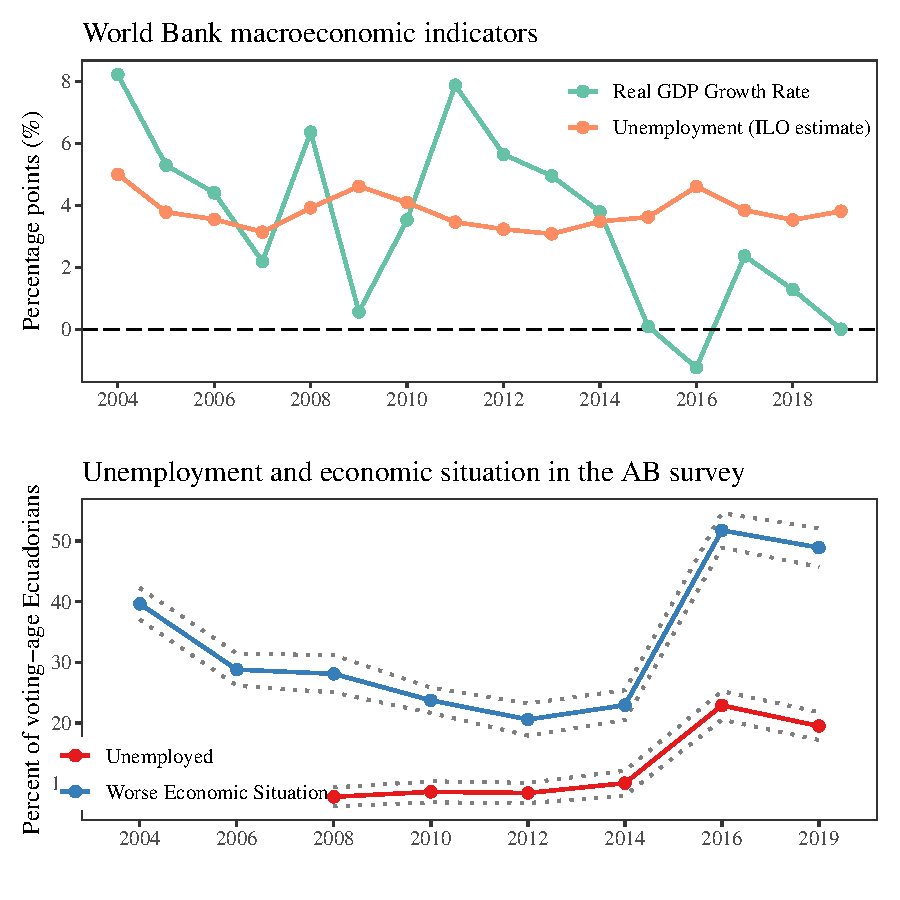
\includegraphics[width=\maxwidth]{figure/econ_graph-1} 

}


\end{knitrout}
\textbf{Note:} Time series line graphs showing key economic indicators for the country between 2004 and 2019. Real GDP growth and unemployment rates extracted from the World Bank's World Development Indicators. WTI oil barrel prices extracted from FRED. The rest are estimates computed with the open-access AB databases, which include 95\% confidence intervals adjusted for design effects. See \hyperref[app:first]{Appendix A} for details on calculations. Figure prepared by the author. 
\end{minipage}}
\end{center}
\end{figure}

Figure \ref{fig:ecua_pol} shows several indicators of public opinion in the country. The AB data shows that indeed the President reached an all-time high popularity in 2014 and then a severe drop in 2016. This is seen through the percent of people who approve the President's job performance and the percent who report confidence in him. Another notable change in the political landscape of this period is the way that voting-age population identified politically. There was a notable increase of the people who identified as the \enquote{right} of the political wings, while those who identified with the \enquote{left} did not see significant changes.

% Methodology Child Document


% Methodology .Rnw File


\section{Methodology}
\label{sec:methodology} % Label the section to cross-reference later.

The AmericasBarometer (AB) survey from the Latin American Public Opinion project is used in this paper to investigate the corruption tolerance increase in Ecuador. This survey was administered in Ecuador and several other Latin American countries from 2004 to 2019, at mostly two-year intervals. It asks about public opinion matters, including democracy, corruption, among others. The open-access AB databases available in the LAPOP \href{https://www.vanderbilt.edu/lapop/data-access.php}{website} are used for the empirical models. Table \ref{tab:descrip} presents descriptive statistics for all variables used.

% Here I will create a descriptive table including averages (and proportions) by year.
% This table is a bit difficult to construct because of its survey-weighted statistics and the rather complex structure, which is why I created it using Excel, exporting the results from calculations done in R.
\begin{table}[htbp!]
\onehalfspacing
\begin{center}
\caption{Descriptive statistics for all variables}
\label{tab:descrip}
\begin{tabular}{llcccc}
\toprule
\multicolumn{1}{c}{\multirow{2}{*}{Variable}} & \multirow{2}{*}{\begin{tabular}[c]{@{}l@{}} Question code \end{tabular}} & \multicolumn{2}{c}{2014}  & \multicolumn{2}{c}{2016}  \\ 
\cmidrule(l{3pt}r{3pt}){3-4} \cmidrule(l{3pt}r{3pt}){5-6}
\multicolumn{1}{c}{}                          &                                                                                         & Est. & SE & Est. & SE \\ \midrule
Corruption tolerance                          & EXC18                                                                                   & 13.59    & 1.39           & 27.18    & 1.21           \\
Unemployment                                  & OCUP4A                                                                                  & 10.06    & 1.04           & 22.89    & 1.2            \\
Confidence in the President                   & B21A                                                                                    & 69.01    & 1.77           & 49.64    & 1.49           \\
Approval of the President                     & M1                                                                                      & 70.26    & 1.57           & 55.41    & 1.43           \\
Economic situation (Worse)                            & IDIO2                                                                                   & 22.93    & 1.26           & 51.76    & 1.45           \\
No political wing                             & L1                                                                                      & 21.49    & 2.11           & 8.67     & 0.74           \\
Center                                        & L1                                                                                      & 42.58    & 1.92           & 45.7     & 1.49           \\
Left                                          & L1                                                                                      & 22.23    & 1.25           & 22.46    & 1.24           \\
Right                                         & L1                                                                                      & 13.7     & 1.16           & 23.17    & 1.15           \\
Women                                         & Q1                                                                                      & 50.37    & 0.34           & 50.29    & 0.3            \\
Age                                           & Q2                                                                                      & 39.41    & 0.17           & 38.64    & 0.22           \\
Years of education                            & ED                                                                                      & 10.67    & 0.15           & 11.43    & 0.14           \\
Urban                                         & UR                                                                                      & 65.21    & 4.11           & 66.41    & 4.07           \\
External political efficacy                   & EFF1                                                                                    & 35.31    & 1.69           & 41.93    & 1.33           \\
Internal political efficacy                   & EFF2                                                                                    & 38.55    & 1.58           & 41.49    & 1.34           \\
Participated in a protest                     & PROT3                                                                                   & 6.82     & 0.89           & 4.67     & 0.55           \\
Interest in politics & POL1 & 33.45 & 1.63 & 32.29 & 1.35 \\
Perceives corruption                          & EXC7, EXC7NEW                                                                           & 70.29    & 1.74           & 83.49    & 0.97           \\
Exposed to corruption                         & EXC 2,6,11,13,14,15,16                                                                  & 26.97    & 2.01           & 27.69    & 1.23           \\ 
\bottomrule
\end{tabular}
\end{center}
Descriptive statistics table with estimates (Est.) and robust standard errors (SE), where age, years of education and the external and internal political efficacies are arithmetic means. All other variables are percentages, calculated for 2014 and 2016. Standard errors are adjusted for survey-design effects. Data is from the open-access AmericasBarometer.
\end{table}

The empirical models estimated in this study will use the 2014 and 2016 rounds of the AB in Ecuador, with $n_{2014}=1489$ and $n_{2016}= 1545$. The survey is based on a multi-stage national probability design. The survey-design adjusted errors for each of these surveys are $\pm 2.5\%$ and $\pm 1.9\%$, respectively (\cite{LAPOP.2014}; \cite{LAPOP.2017}). Both surveys are self-weighted, however, 95\% confidence intervals for the descriptive statistics which are adjusted for survey-design effects are presented when relevant. 

The empirical analysis is concerned with the \emph{EXC18} question: \enquote{Do you think given the way things are, sometimes paying a bribe is justified?} \parencite[p.96]{Moscoso.2018}, originally asked in Spanish. The question has been asked in all survey rounds in Ecuador and is the last one after a set of questions regarding corruption exposure and perception. This variable ($ctol$) is equal to 1 when the respondent answers \enquote{Yes}, 0 when the answer is \enquote{No} and dropped from the model otherwise. All models have $ctol$ as the explained variable and responses to other questions are used as regressors. 

In order to identify the changes in behavior which led to the increase, the survey rounds are pooled and the following general model is estimated: 

\begin{equation}
\label{eqn:genmod}
P(ctol = 1 | \textbf{\textit{X}} \hspace{0.04cm}) = G (\textbf{\textit{X}} \theta ) = G \left[ \beta_0 + \delta_0 y_{16} + \textbf{\textit{R}}'\beta + \delta_1 (y_{16} \cdot x^*) \right]
\end{equation}

where $\textbf{\textit{R}}$ is a vector of controls and $x^*$ is a key regressor whose change across time may have significantly influenced the rise of $ctol$ between 2014 and 2016. This key regressor is interacted with a year dummy, $y_{16}$, which equals unity for 2016 observations. The complete regressors' vector $\textbf{\textit{X}}$ includes all variables in $\textbf{\textit{R}}$, the key regressor $x^*$ and the interaction term. The parameters vector $\theta$ includes the vector $\beta$ as well as $\beta_0$, $\delta_0$ and $\delta_1$. $G$ is the link function; in this paper I follow the literature and use a logistic function as $G$. 

Consider the partial effect of the key regressor $x^*$ on $P(ctol =1| \textbf{\textit{X}})$:
\begin{equation}
\label{eqn:keype}
\dfrac{\partial P(ctol = 1 | \textbf{\textit{X}} \hspace{0.04cm})}{\partial x^*} = \dfrac{\partial G}{\partial \theta} \cdot 
\dfrac{\partial \theta}{\partial x^*} = \dfrac{\partial G}{\partial \theta} \cdot (\beta_{x^*}+ \delta_1 y_{16})
\end{equation}

The parameter $\delta_1$ would then measure the ceteris paribus effect of a change in the key regressor $x^*$ from 2014 to 2016 in $ctol$. Therefore, the coefficient of interest in this study is $\widehat{\delta}_1$. If there has been a change in 2016 in $x^*$ which significantly influences corruption tolerance, $\widehat{\delta_1}$ should be statistically significant. Further, a $\widehat{\delta}_1$ coefficient not statistically different from zero would mean that individuals with and without this key characteristic are equally likely to justify corruption across time. 

Average partial effects tables are shown for all models. I use survey-weighting to adjust for complex-survey design effects, as suggested by \textcite{Castorena.2021}. Since the sample is self-weighted, survey-weighting does not affect magnitudes, only standard errors.

% Results 1 Child Document


% Results II .Rnw File

\section{Results}
\label{sec:results}
Section \ref{sec:background} identified some key events which happenned at the same time of the corruption tolerance increase. Two economic variables observed at the individual level through the AB significantly changed during this period: the percent of people who report a worse economic situation as well as unemployment. Variables which proxy attitudes in the political landscape have also significantly changed: the percentage of people who confide in the President, the percentage who approve the President's job and also the percentage of people who identify with the political right wing. These variables where used for simple empirical models, which follow the equation below.

\begin{equation}
\label{eqn:simplemod}
P(ctol = 1 | \textbf{\textit{X}} \hspace{0.04cm}) = G \left[ \beta_0 + \delta_0 y_{16} + \beta_1 x^* + \delta_1 (y_{16} \cdot x^*)\right]
\end{equation}
where the key regressor $x^*$ can be: a dummy variable set to unity for respondents who answered that their economic situation is worse (Model 1), a dummy variable set to unity for those who report being unemployed (Model 2), a discrete variable with numbers 1-7, where higher values imply a higher degree of confidence in the President (Model 3), a discrete variable with numbers 1-5, with higher numbers implying a higher rating of the President's job performance (Model 4) or a discrete variable with numbers from 1-10 where 1 is the extreme left and 10 is the extreme right (Model 5). 

Table \ref{tab:simplemodel} presents coefficients of the logistic model for Equation \ref{eqn:simplemod} and Table \ref{tab:apesimp} presents their associated average partial effects. It is show that an unemployed person is 5.9\% more likely to justify corruption. Additionally, a respondent who answered one number higher for an increased degree of confidence in the President was 2.4\% less likely to justify corruption. Finally, a person who rated the President's job performance one unit higher was 4.4\% less likely to justify corruption. All other partial effects are not significant.

% Now, I'll make the table with modelsummary from the sourced stuff. 
\begin{table}[htbp]
\caption{Logit coefficients for baseline models}
\label{tab:simplemodel}

\begin{tabular}[t]{lccccc}
\toprule
  & Model 1 & Model 2 & Model 3 & Model 4 & Model 5\\
\midrule
Constant & \num{-1.894}*** & \num{-1.989}*** & \num{-0.455}** & \num{0.553} & \num{-1.527}***\\
 & (\num{0.127}) & (\num{0.110}) & (\num{0.208}) & (\num{0.362}) & (\num{0.196})\\
2016 Dummy & \num{0.848}*** & \num{1.001}*** & \num{-0.188} & \num{-1.251}*** & \num{0.278}\\
 & (\num{0.158}) & (\num{0.132}) & (\num{0.238}) & (\num{0.415}) & (\num{0.234})\\
Worse Economic Situation & \num{0.131} &  &  &  & \\
 & (\num{0.169}) &  &  &  & \\
Unemployment &  & \num{1.015}*** &  &  & \\
 &  & (\num{0.205}) &  &  & \\
Confidence in President &  &  & \num{-0.288}*** &  & \\
 &  &  & (\num{0.037}) &  & \\
Approval of Pres. Performance &  &  &  & \num{-0.648}*** & \\
 &  &  &  & (\num{0.096}) & \\
Political Wing &  &  &  &  & \num{-0.047}\\
 &  &  &  &  & (\num{0.038})\\
Econ. Situation Interaction & \num{-0.025} &  &  &  & \\
 & (\num{0.197}) &  &  &  & \\
Unemployment Interaction &  & \num{-1.005}*** &  &  & \\
 &  & (\num{0.256}) &  &  & \\
Pres. Confidence Interaction &  &  & \num{0.206}*** &  & \\
 &  &  & (\num{0.044}) &  & \\
Pres. Approval Interaction &  &  &  & \num{0.568}*** & \\
 &  &  &  & (\num{0.111}) & \\
Pol. Wing Interaction &  &  &  &  & \num{0.095}**\\
 &  &  &  &  & (\num{0.043})\\
\midrule
$N$ & \num{2948} & \num{2950} & \num{2944} & \num{2941} & \num{2535}\\
AIC & \num{2893.64} & \num{2889.04} & \num{2848.57} & \num{2844.82} & \num{2574.81}\\
BIC & \num{2926.37} & \num{2920.98} & \num{2881.80} & \num{2876.65} & \num{2606.10}\\
\bottomrule
\end{tabular}


\vspace{0.25cm}
Logit coefficients of baseline models (Equation \ref{eqn:simplemod}) with design-adjusted std. errors.\\
*$p$ < 0.1, **$p$< 0.05, ***$p$ < 0.01.
\end{table}

% Do the APE table
\begin{table}[htbp]
\caption{Average partial effects for logit models in Table \ref{tab:simplemodel}}
\label{tab:apesimp}

\begin{tabular}[t]{lccccc}
\toprule
  & Model 1 & Model 2 & Model 3 & Model 4 & Model 5\\
\midrule
2016 Dummy & \num{0.131}*** & \num{0.126}*** & \num{0.109}*** & \num{0.117}*** & \num{0.124}***\\
 & (\num{0.020}) & (\num{0.019}) & (\num{0.019}) & (\num{0.019}) & (\num{0.020})\\
Worse Economic Situation & \num{0.018} &  &  &  & \\
 & (\num{0.014}) &  &  &  & \\
Unemployment &  & \num{0.058}*** &  &  & \\
 &  & (\num{0.020}) &  &  & \\
Confidence in President &  &  & \num{-0.024}*** &  & \\
 &  &  & (\num{0.003}) &  & \\
Approval of Pres. Performance &  &  &  & \num{-0.044}*** & \\
 &  &  &  & (\num{0.008}) & \\
Political Wing &  &  &  &  & \num{0.003}\\
 &  &  &  &  & (\num{0.003})\\
\midrule
$N$ & \num{2948} & \num{2950} & \num{2944} & \num{2941} & \num{2535}\\
\bottomrule
\end{tabular}


\vspace{0.25cm}
Average partial effects for models in Table \ref{tab:simplemodel}, with design-adjusted std. errors.\\
*$p$ < 0.1, **$p$< 0.05, ***$p$ < 0.01.
\end{table}

Consider the logit coefficients in Table \ref{tab:simplemodel}. The coefficient for the year dummy confirms the significance of the corruption tolerance increase in 2016, which is lost when considering interaction terms with confidence in the President, and actually has a negative sign with the other political variables. The inclusion of unemployment and economic situation do not eliminate the significance of the year dummy. Model 1 suggests that a person who reports having a worse economic situation does not tolerate corruption differently than those who report a same or equal economic situation. According to Model 2, respondents who were unemployed were more likely to justify corruption than those who were not unemployed\footnote{In this case, not being unemployed means either being employed, salary and hours worked notwithstanding, and also not being in the labor force (students, rentists, among others). Results all throughout this paper are robust to including an employment variable.} The interaction term in this model has a negative sign, which shows that the effect of unemployment in 2016 was less than the effect in 2014, meaning unemployed people actually justified corruption less after political instability set in. 

Models 3 and 4 display the same relationship: people who either trust or approve of the President in a higher degree also tolerate corruption less. A more zealous supporter of the regime believed bribes were not justified; however, this appears to change for 2016. The interaction terms for both variables are significant and positive: in 2016 supporters started to justify corruption more. This could explain the jump in corruption tolerance as regime support eroded in 2016, which meant that the number of non-supporters was higher and these respondents justified corruption more than supporters. Also, the supporters that remained started to justify bribes to a higher degree. In Model 3, the significance of the year dummy is lost, while in Model 4 its sign reversed.

The coefficients in Model 5 show that a person who identifies closer to the political right does not justify corruption more or less relative to those identifying closer to the political left. However, the interaction term shows that people answering higher values of this variable justified corruption more in 2016. Once again, the significance of the year dummy is lost when considering this variable. With a higher number of respondents identifying with the political right wing, who appear to justify corruption more, it would be understood how overall corruption tolerance increased.

% I need to draw the graph which shows the visual differences between groups and their corruption tolerance

% Now I do the data wrangling needed for this


% Now do the graph
\begin{figure}[htbp]
\begin{knitrout}
\definecolor{shadecolor}{rgb}{0.969, 0.969, 0.969}\color{fgcolor}

{\centering 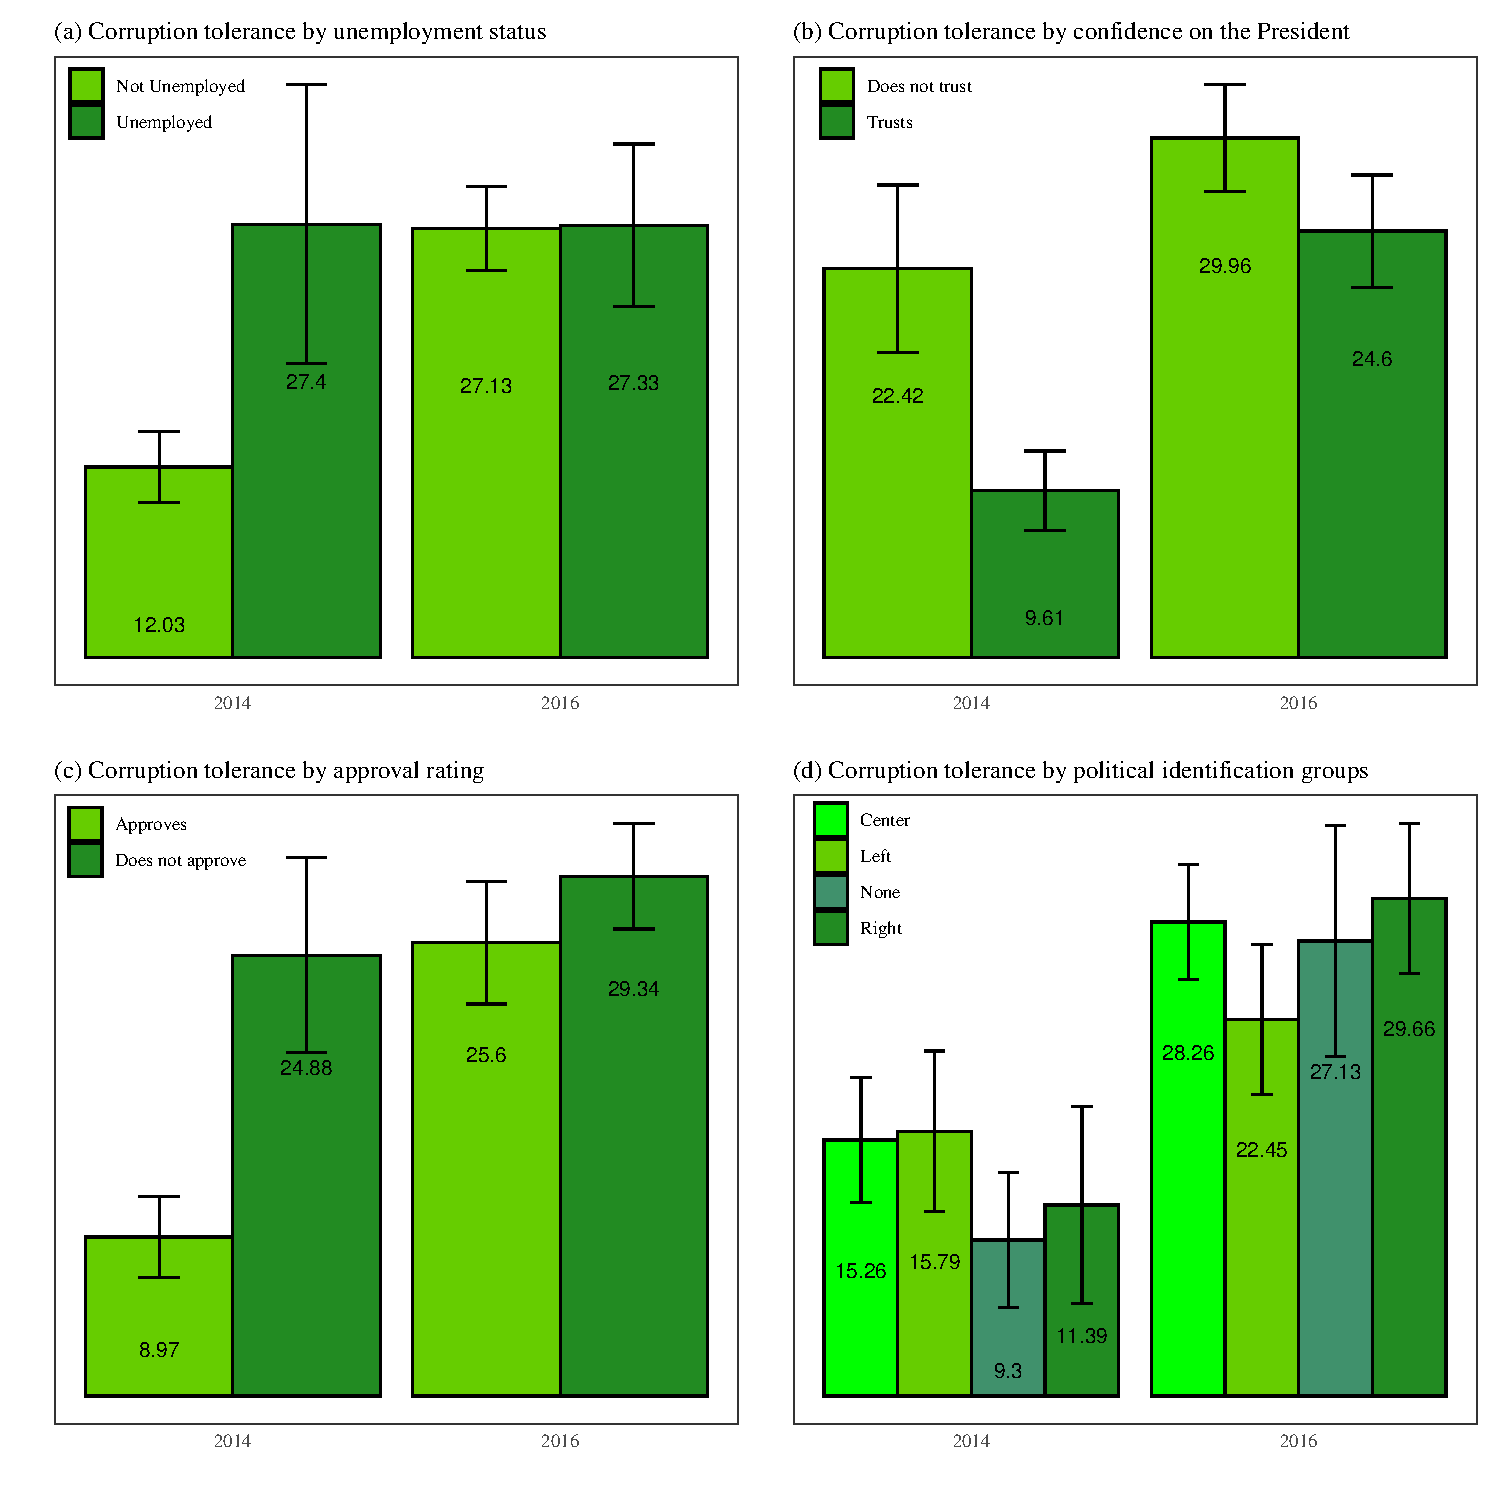
\includegraphics[width=\maxwidth]{figure/difgraph-1} 

}


\end{knitrout}
\caption{Graphical representations of corruption tolerance across key explanatory variables}
\label{fig:difgraph}
Figures show the percent that justify corruption across the groups used as explanatory models in Table \ref{tab:simplemodel}. Error bars represent the 95\% confidence intervals adjusted for design effects.
\end{figure}

These findings are supported by Figure \ref{fig:difgraph}. According to panel (a), in 2014, only 12.03\% of those not unemployed justified corruption, while in 2016 this figure increased to 27.03\%, very close to the percentage of unemployed people who justified it in 2016. The time difference between these point estimates is not statistically significant, which means that in 2016 the effect of unemployment in corruption tolerance approached zero. Thus, Figure \ref{fig:difgraph} along with Model 2 of Table \ref{tab:simplemodel} show that it was not the unemployed who started to justify corruption less, it was that the people who were not unemployed started to justify it more. Panels (b) and (c) of Figure \ref{fig:difgraph} show that the percentage of people who either confided in or approved the President and justified corruption increased significantly  between 2014 and 2016. This means that the negative effect of supporting the executive in 2016 was smaller than in 2014, as confirmed by the interaction term in Models 3 and 4 of Table \ref{tab:simplemodel}. In panel (d) of Figure \ref{fig:difgraph}, where four different political groups are considered: the left, right, center and those who did not answer the question. All four groups saw increases in the percent of group members who justify corruption. All increases in corruption tolerance are significant, except for those who identify with the left wing. This is consistent with the coefficient sign seen in Model 5 for the political score variable. 



\end{document}
